\documentclass[ngerman,pstricks,border=12pt]{standalone}
% --- Pakete einbinden
\input{01_PaketeEinstellungen.tex}
\begin{document}
\begin{figure}[H]
\centering
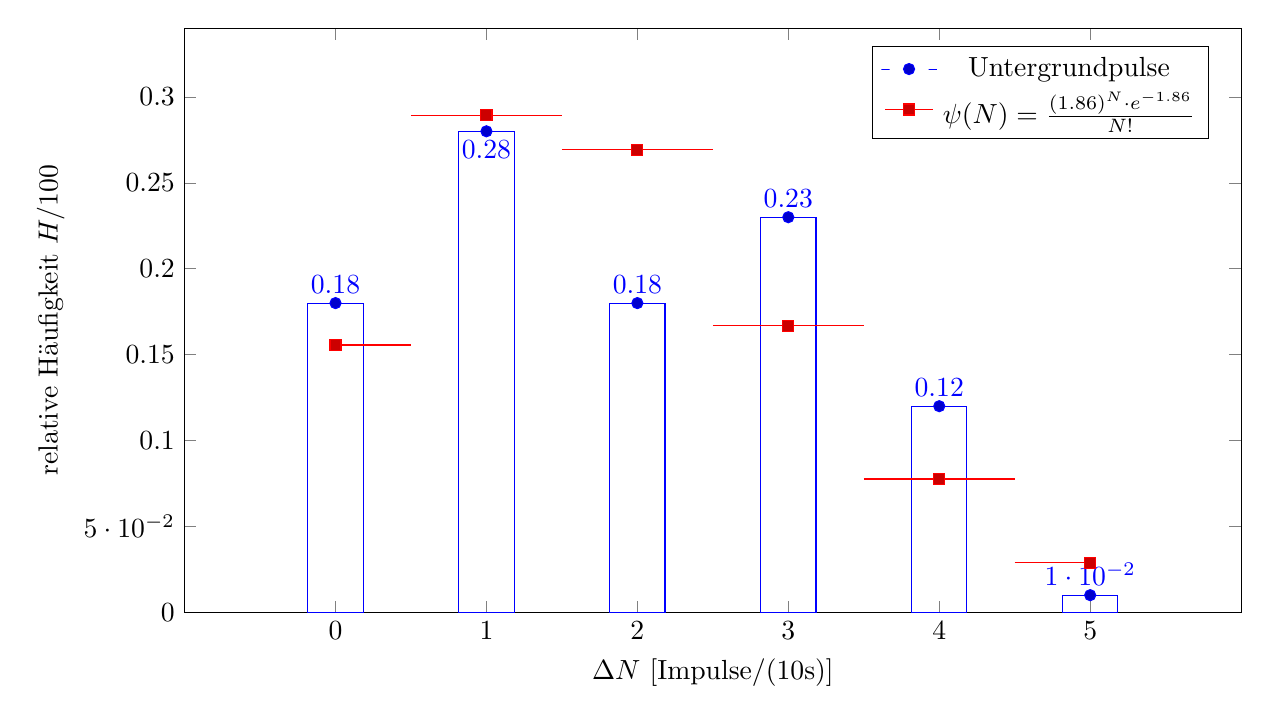
\begin{tikzpicture}
  \begin{axis}[
    width=15 cm,
    height=9 cm,
    xmin=-1, xmax=6,
    ymin=0, ymax=0.34,
    xlabel={$\Delta N$ [Impulse/(\SI{10}{s})]},
    ylabel={relative Häufigkeit $H/100$},
    domain=0:5,
		samples=6,
    legend entries={Untergrundpulse, $\psi(N)=\frac{(\num{1.86})^N\cdot e^{-\num{1.86}}}{N!}$},
    legend pos=north east,
		bar width=20pt,
		xtick={0,1,...,5}
  ]
  \addplot+[ybar, nodes near coords, forget plot] plot coordinates {
		(0,0.18)	(2,0.18)	(3,0.23)	(4,0.12)	(5,0.01)
		};
	\addplot+[ybar, nodes near coords, every node near coord/.append style={anchor=north}] plot coordinates {
		(1,0.28)
		};
	\addplot+[jump mark mid] {(1.86)^x*e^(-1.86)/factorial(x)};
  \end{axis}
\end{tikzpicture}
\label{fig:untergrundrelativ}
\end{figure}
\end{document}